\documentclass[11pt,a4paper]{article}

\usepackage[utf8]{inputenc}
\usepackage[T1]{fontenc}
\usepackage[croatian]{babel}
\usepackage[a4paper,margin=2.2cm]{geometry}
\usepackage{microtype}
\usepackage{lmodern}
\usepackage{booktabs}
\usepackage{longtable}
\usepackage{array}
\usepackage{tabularx}
\usepackage{amssymb}
\usepackage{xcolor}
\usepackage{colortbl}
\usepackage{enumitem}
\usepackage{titlesec}
\usepackage[hidelinks,colorlinks=true,linkcolor=blue!50!black,urlcolor=blue!50!black]{hyperref}
\usepackage{listings}
\usepackage{fancyhdr}
\usepackage{tikz}
\usetikzlibrary{calc,positioning,arrows.meta,shapes.geometric}

\definecolor{cellhigh}{RGB}{255,238,221}
\definecolor{cellmed}{RGB}{255,250,222}
\definecolor{celllow}{RGB}{226,245,229}
\definecolor{headergray}{RGB}{60,60,60}
\definecolor{coderule}{RGB}{200,200,200}
\definecolor{daygray}{RGB}{45,55,72}
\definecolor{daylight}{RGB}{237,242,247}
\definecolor{shellbg}{RGB}{30,30,30}
\definecolor{shellfg}{RGB}{230,230,230}

\lstdefinestyle{Rstyle}{
  basicstyle=\ttfamily\footnotesize,
  breaklines=true,
  frame=single,
  rulecolor=\color{coderule},
  framesep=4pt,
  xleftmargin=4pt,
  xrightmargin=4pt,
  showstringspaces=false,
  language=R,
  keywordstyle=\color{blue!60!black}\bfseries,
  commentstyle=\color{green!40!black}\itshape,
  stringstyle=\color{red!60!black}
}
\lstdefinestyle{Stanstyle}{
  basicstyle=\ttfamily\footnotesize,
  breaklines=true,
  frame=single,
  rulecolor=\color{coderule},
  framesep=4pt,
  xleftmargin=4pt,
  xrightmargin=4pt,
  showstringspaces=false
}
\lstdefinestyle{Shellstyle}{
  basicstyle=\ttfamily\footnotesize\color{shellfg},
  backgroundcolor=\color{shellbg},
  breaklines=true,
  frame=single,
  framesep=4pt,
  xleftmargin=4pt,
  xrightmargin=4pt,
  showstringspaces=false
}
\lstset{style=Rstyle}

\titleformat{\section}{\color{headergray}\Large\bfseries}{\thesection.}{0.6em}{}
\titleformat{\subsection}{\color{headergray}\large\bfseries}{\thesubsection}{0.6em}{}
\titleformat{\subsubsection}{\color{headergray}\normalsize\bfseries}{\thesubsubsection}{0.6em}{}

\pagestyle{fancy}
\fancyhf{}
\fancyhead[L]{\small BayesianDEB --- JSS revizija: plan rada}
\fancyhead[R]{\small \today}
\fancyfoot[C]{\thepage}
\renewcommand{\headrulewidth}{0.3pt}

\newcommand{\dayhead}[2]{%
  \vspace{0.6em}\par\noindent%
  \colorbox{daygray}{\color{white}\bfseries\strut\;DAN #1\;}\;%
  \colorbox{daylight}{\color{daygray}\strut\;#2\;}\par\vspace{0.4em}%
}
\newcommand{\task}[2]{\par\vspace{0.3em}\noindent\textbf{[#1]}\; #2\par}
\newcommand{\file}[1]{\texttt{\small #1}}
\newcommand{\fn}[1]{\texttt{\small #1()}}
\newcommand{\code}[1]{\texttt{\small #1}}

\title{\textbf{BayesianDEB --- Detaljan plan rada \\ \large JSS revizija (0.1.4 $\rightarrow$ 0.2.0)}}
\author{Branimir K.~Hackenberger \\ \small SCIOM d.o.o., \texttt{branimir@sciom.hr}}
\date{\today}

\begin{document}
\maketitle
\thispagestyle{fancy}

\tableofcontents
\bigskip\hrule\bigskip

\section{Opcija A i radne predispozicije}

Ovaj plan pretpostavlja:
\begin{itemize}[leftmargin=1.4em,nosep]
  \item Radnu granu \code{git checkout -b jss-revision} iz \code{main} (0.1.4).
  \item Da je \code{cmdstanr} već instaliran lokalno
    (\code{cmdstanr::cmdstan\_path()} ne-prazan).
  \item Da \fn{R CMD check --as-cran} trenutno prolazi 0/0/1
    NOTE-om (\texttt{Additional\_repositories}).
  \item Po završetku Faze 1, \fn{devtools::test()} mora ostati zelen
    (901+ testova).
  \item Nakon svake izmjene dokumentacije: \fn{devtools::document()} +
    \fn{devtools::check()}.
\end{itemize}

\paragraph{Radne pretpostavke vremena.} Procjena pretpostavlja
8-satne radne dane.  Faze su sekvencijalne, ali se zahvati
\emph{unutar} dana mogu paralelizirati ako više osoba radi.

\paragraph{Verzija.} Skok na \textbf{0.2.0} odmah u prvom commitu
(\file{DESCRIPTION}: \code{Version: 0.2.0}).

\section{Pregled --- Gantt}

\begin{center}
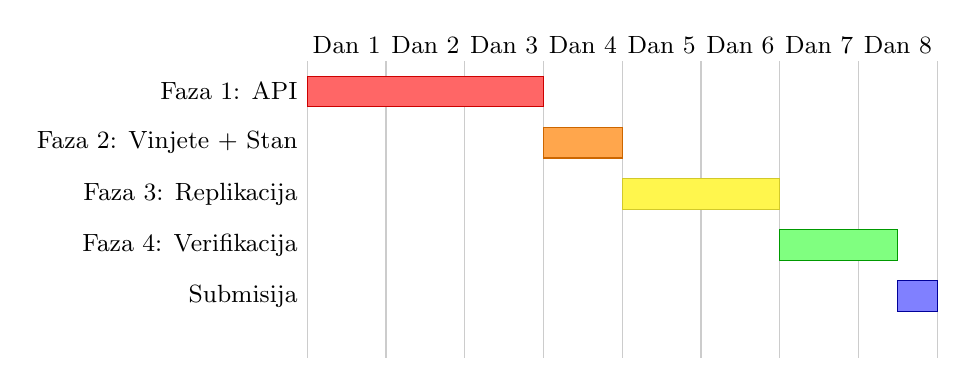
\begin{tikzpicture}[x=1.0cm,y=0.65cm]
  % grid
  \foreach \x in {0,1,...,8} \draw[gray!40] (\x,-0.2) -- (\x,5.6);
  \foreach \x/\d in {0/1,1/2,2/3,3/4,4/5,5/6,6/7,7/8}
    \node[font=\small] at (\x+0.5,5.9) {Dan~\d};
  % labels
  \node[anchor=east,font=\small] at (0,5.0) {Faza 1: API};
  \node[anchor=east,font=\small] at (0,4.0) {Faza 2: Vinjete + Stan};
  \node[anchor=east,font=\small] at (0,3.0) {Faza 3: Replikacija};
  \node[anchor=east,font=\small] at (0,2.0) {Faza 4: Verifikacija};
  \node[anchor=east,font=\small] at (0,1.0) {Submisija};
  % bars
  \draw[fill=red!60,draw=red!80!black]   (0,4.7) rectangle (3,5.3);
  \draw[fill=orange!70,draw=orange!80!black] (3,3.7) rectangle (4,4.3);
  \draw[fill=yellow!70,draw=yellow!80!black] (4,2.7) rectangle (6,3.3);
  \draw[fill=green!50,draw=green!60!black]   (6,1.7) rectangle (7.5,2.3);
  \draw[fill=blue!50,draw=blue!60!black]     (7.5,0.7) rectangle (8,1.3);
\end{tikzpicture}
\end{center}

\section{Faza 1 --- API stabilizacija (Dani 1--3)}

\dayhead{1}{API klase: \texttt{bdeb\_diagnostics} + \texttt{bdeb\_prediction}}

\subsubsection*{[B6] Restruktura \texttt{bdeb\_diagnose} u klasificirani tip
(3{,}5--4 h)}

\paragraph{Cilj.} \fn{bdeb\_diagnose} treba vratiti S3 objekt klase
\code{bdeb\_diagnostics}, a sav ispis seliti u
\code{print.bdeb\_diagnostics}.

\paragraph{Datoteke.} \file{R/diagnostics.R}, \file{NAMESPACE}
(auto), \file{man/bdeb\_diagnose.Rd} (auto),
\file{tests/testthat/test-diagnostics.R}.

\paragraph{Implementacija.}

\begin{lstlisting}
#' @export
bdeb_diagnose <- function(fit, pars = NULL) {
  if (!inherits(fit, "bdeb_fit"))
    cli::cli_abort("{.arg fit} must be a {.cls bdeb_fit} object.")

  diag  <- fit$fit$diagnostic_summary(quiet = TRUE)
  draws <- posterior::as_draws_df(fit$fit$draws())

  if (is.null(pars)) {
    all_vars <- posterior::variables(draws)
    pars <- all_vars[!grepl("^(log_lik|L_rep|R_rep|lp__|p_Am_new)",
                            all_vars)]
  }

  summ <- posterior::summarise_draws(
    posterior::subset_draws(draws, variable = pars),
    "mean", "sd", "median",
    "q5"  = ~ quantile(.x, 0.05),
    "q95" = ~ quantile(.x, 0.95),
    "rhat", "ess_bulk", "ess_tail"
  )

  out <- list(
    n_divergent     = sum(diag$num_divergent),
    n_max_treedepth = sum(diag$num_max_treedepth),
    ebfmi           = diag$ebfmi,
    summary         = summ,
    pars            = pars,
    model_type      = fit$model$type
  )
  structure(out, class = "bdeb_diagnostics")
}

#' @export
print.bdeb_diagnostics <- function(x, ...) {
  cli::cli_h2("BDEB Diagnostics ({x$model_type})")
  if (x$n_divergent > 0)
    cli::cli_alert_danger("Divergent transitions: {x$n_divergent}")
  else
    cli::cli_alert_success("No divergent transitions.")
  if (x$n_max_treedepth > 0)
    cli::cli_alert_warning("Max treedepth: {x$n_max_treedepth} times.")
  else
    cli::cli_alert_success("Treedepth OK.")
  low <- which(x$ebfmi < 0.3)
  if (length(low))
    cli::cli_alert_warning("Low E-BFMI for chain(s): {low}")
  else
    cli::cli_alert_success("E-BFMI OK (all > 0.3).")
  invisible(x)
}

#' @export
summary.bdeb_diagnostics <- function(object, ...) {
  bad_rhat <- object$summary$variable[
    !is.na(object$summary$rhat) & object$summary$rhat > 1.01]
  low_ess  <- object$summary$variable[
    !is.na(object$summary$ess_bulk) & object$summary$ess_bulk < 400]
  out <- list(
    n_divergent     = object$n_divergent,
    n_max_treedepth = object$n_max_treedepth,
    n_bad_rhat      = length(bad_rhat),
    n_low_ess       = length(low_ess),
    bad_rhat        = bad_rhat,
    low_ess         = low_ess,
    table           = object$summary
  )
  structure(out, class = "summary.bdeb_diagnostics")
}

#' @export
plot.bdeb_diagnostics <- function(x, type = c("rhat", "ess"), ...) {
  type <- match.arg(type)
  df <- as.data.frame(x$summary)
  if (type == "rhat") {
    ggplot2::ggplot(df, ggplot2::aes(x = .data$rhat,
                                     y = .data$variable)) +
      ggplot2::geom_point() +
      ggplot2::geom_vline(xintercept = 1.01, linetype = "dashed") +
      ggplot2::theme_minimal()
  } else {
    ggplot2::ggplot(df, ggplot2::aes(x = .data$ess_bulk,
                                     y = .data$variable)) +
      ggplot2::geom_point() +
      ggplot2::geom_vline(xintercept = 400, linetype = "dashed") +
      ggplot2::theme_minimal()
  }
}
\end{lstlisting}

\paragraph{Provjere.}
\begin{lstlisting}[style=Shellstyle]
Rscript -e 'devtools::document()'
Rscript -e 'devtools::test(filter = "diagnostics")'
\end{lstlisting}

\paragraph{Test (dodati).}
\begin{lstlisting}
test_that("bdeb_diagnose returns bdeb_diagnostics object", {
  fit <- readRDS(test_path("fixtures/fit_individual.rds"))
  d <- bdeb_diagnose(fit)
  expect_s3_class(d, "bdeb_diagnostics")
  expect_named(d, c("n_divergent","n_max_treedepth","ebfmi",
                    "summary","pars","model_type"))
  expect_invisible(print(d))
  expect_s3_class(plot(d, "rhat"), "ggplot")
})
\end{lstlisting}

\subsubsection*{[B5] Klasa \texttt{bdeb\_prediction} -- print + summary
(3 h)}

\paragraph{Cilj.} \fn{predict.bdeb\_fit} već vraća objekt klase
\code{bdeb\_prediction} (provjeriti), ali nedostaju \code{print} i
\code{summary} metode.

\paragraph{Datoteke.} \file{R/ppc.R} (gdje je
\code{predict.bdeb\_fit}), \file{R/plot.R} (\code{plot.bdeb\_prediction}
već postoji).

\paragraph{Implementacija.}

\begin{lstlisting}
#' @export
print.bdeb_prediction <- function(x, ...) {
  cli::cli_h2("BDEB Prediction")
  cli::cli_li("Model type: {.val {x$model_type %||% 'unknown'}}")
  cli::cli_li("Draws: {.val {NROW(x$draws %||% x$L_hat)}}")
  cli::cli_li("Time points: {.val {NROW(x$time)}}")
  cli::cli_alert_info("Use {.code summary(x)} for credible intervals,
                      or {.code plot(x)} for trajectory.")
  invisible(x)
}

#' @export
summary.bdeb_prediction <- function(object, prob = 0.90, ...) {
  alpha <- (1 - prob) / 2
  qs    <- c(alpha, 0.5, 1 - alpha)
  q_fn  <- function(M) {
    apply(M, 2, function(col) stats::quantile(col, qs, na.rm = TRUE))
  }
  L <- if (!is.null(object$L_hat)) object$L_hat
       else object$draws
  qmat <- q_fn(L)
  out <- data.frame(
    time   = object$time,
    lower  = qmat[1, ],
    median = qmat[2, ],
    upper  = qmat[3, ]
  )
  structure(out,
            class = c("summary.bdeb_prediction", "data.frame"),
            prob  = prob)
}

#' @export
print.summary.bdeb_prediction <- function(x, ...) {
  cli::cli_h3("Prediction summary ({attr(x, 'prob') * 100}% CrI)")
  print.data.frame(head(as.data.frame(x), 10), row.names = FALSE)
  if (NROW(x) > 10)
    cli::cli_alert_info("[... {NROW(x) - 10} more rows ...]")
  invisible(x)
}
\end{lstlisting}

\paragraph{Provjera.}
\begin{lstlisting}[style=Shellstyle]
Rscript -e 'pkgload::load_all(); set.seed(1)
fit <- readRDS("tests/testthat/fixtures/fit_individual.rds")
p <- predict(fit, n_draws = 50)
print(p); summary(p); plot(p)'
\end{lstlisting}

\paragraph{Definition of done (Dan 1).}
\begin{itemize}[leftmargin=1.4em,nosep]
  \item \code{methods(class = "bdeb\_diagnostics")} ispisuje
    \emph{plot, print, summary}.
  \item \code{methods(class = "bdeb\_prediction")} ispisuje
    \emph{plot, print, summary}.
  \item Testovi prolaze.
  \item Commit: \code{feat: bdeb\_diagnostics class + bdeb\_prediction
    methods (B5, B6)}.
\end{itemize}

\dayhead{2}{Generic-i: \texttt{bdeb\_summary} deprecation,
\texttt{bdeb\_derived}, lm-stilske metode}

\subsubsection*{[B9] Deprekacija \texttt{bdeb\_summary} (0{,}5 h)}

\begin{lstlisting}
#' @export
bdeb_summary <- function(fit, pars = NULL, prob = 0.90, ...) {
  .Deprecated("summary",
              package = "BayesianDEB",
              msg = "bdeb_summary() is deprecated; use summary() instead.")
  summary(fit, pars = pars, prob = prob, ...)
}
\end{lstlisting}

\noindent Ostaviti u 0.2.0; ukloniti u 0.3.0.

\subsubsection*{[B7] \texttt{bdeb\_derived} kao S3 metoda (2--3 h)}

\paragraph{Cilj.} Eksportirati \code{generic + method} pattern, ne
mijenjati javno ime.

\begin{lstlisting}
#' @export
bdeb_derived <- function(x, ...) UseMethod("bdeb_derived")

#' @export
bdeb_derived.default <- function(x, ...) {
  cli::cli_abort("No bdeb_derived() method for class
                  {.cls {class(x)[1]}}.")
}

#' @export
bdeb_derived.bdeb_fit <- function(x, ...) {
  ## premjesti dosadasnje tijelo bdeb_derived() ovamo
}
\end{lstlisting}

\noindent U \file{NAMESPACE} (auto):
\code{S3method(bdeb\_derived, bdeb\_fit)}.

\subsubsection*{[B8] lm-stilske metode za \texttt{bdeb\_fit} (5--7 h)}

Implementirati u \file{R/methods.R} (nova datoteka):

\begin{lstlisting}
#' @export
confint.bdeb_fit <- function(object, parm = NULL, level = 0.90, ...) {
  alpha <- (1 - level) / 2
  draws <- posterior::as_draws_matrix(object$fit$draws())
  vars  <- if (is.null(parm)) colnames(draws) else parm
  q <- apply(draws[, vars, drop = FALSE], 2,
             stats::quantile, probs = c(alpha, 1 - alpha),
             na.rm = TRUE)
  out <- t(q)
  colnames(out) <- paste0(c(alpha, 1 - alpha) * 100, " %")
  out
}

#' @export
fitted.bdeb_fit <- function(object, ...) {
  draws <- object$fit$draws("L_hat", format = "draws_matrix")
  if (is.null(draws) || NCOL(draws) == 0)
    cli::cli_abort("No L_hat in fit; nothing to extract.")
  apply(draws, 2, stats::median)
}

#' @export
residuals.bdeb_fit <- function(object, type = "response", ...) {
  type <- match.arg(type, c("response", "pearson"))
  fv <- fitted(object)
  y  <- object$model$data$L %||% object$model$data$y
  if (is.null(y))
    cli::cli_abort("No observed response on the fit.")
  r <- y - fv
  if (type == "pearson") {
    sigma <- stats::sd(r)
    if (sigma > 0) r <- r / sigma
  }
  r
}

#' @export
nobs.bdeb_fit <- function(object, ...) {
  length(object$model$data$L %||% object$model$data$y %||% NULL)
}

#' @export
vcov.bdeb_fit <- function(object, parm = NULL, ...) {
  draws <- posterior::as_draws_matrix(object$fit$draws())
  vars  <- if (is.null(parm)) colnames(draws) else parm
  stats::cov(draws[, vars, drop = FALSE])
}

#' @export
logLik.bdeb_fit <- function(object, ...) {
  ll <- try(loo::extract_log_lik(object$fit, merge_chains = TRUE),
            silent = TRUE)
  if (inherits(ll, "try-error"))
    cli::cli_abort("log_lik not available on this fit.")
  out <- sum(matrixStats::colMeans2(ll))
  attr(out, "df")  <- length(object$fit$metadata()$variables)
  attr(out, "nobs") <- nobs(object)
  class(out) <- "logLik"
  out
}
\end{lstlisting}

\paragraph{Roxygen.} Svaku metodu dokumentirati s
\code{@rdname bdeb\_fit-methods} kako bi imala jednu zajedničku Rd.

\paragraph{Test.}
\begin{lstlisting}
test_that("bdeb_fit has lm-style methods", {
  fit <- readRDS(test_path("fixtures/fit_individual.rds"))
  expect_true(is.matrix(confint(fit)))
  expect_true(is.numeric(fitted(fit)))
  expect_true(is.numeric(residuals(fit)))
  expect_gt(nobs(fit), 0)
  expect_true(is.matrix(vcov(fit)))
})
\end{lstlisting}

\paragraph{Definition of done (Dan 2).}
\begin{itemize}[leftmargin=1.4em,nosep]
  \item \code{methods(class = "bdeb\_fit")} sadrži:
    \emph{coef, confint, fitted, logLik, nobs, plot, predict,
    print, residuals, summary, vcov}.
  \item \fn{bdeb\_derived(fit)} radi kao prije; \code{class(fit)} kao
    prije.
  \item Commit: \code{feat: lm-style methods + bdeb\_derived as S3
    method (B7, B8, B9)}.
\end{itemize}

\dayhead{3}{\texttt{bdeb\_data}, \texttt{bdeb\_model},
\texttt{bdeb\_prior}; primjeri; validacija}

\subsubsection*{[B1] \texttt{summary.bdeb\_data}, \texttt{plot.bdeb\_data}
(3--4 h)}

\file{R/data\_prep.R} dodati:

\begin{lstlisting}
#' @export
summary.bdeb_data <- function(object, ...) {
  out <- list(
    n_obs        = NROW(object$growth %||% object$repro),
    n_individuals = length(unique(
      (object$growth %||% object$repro)$id)),
    time_range   = range((object$growth %||% object$repro)$time,
                          na.rm = TRUE),
    has_growth   = !is.null(object$growth),
    has_repro    = !is.null(object$repro),
    f_food       = object$f_food
  )
  if (!is.null(object$conc))
    out$conc_levels <- sort(unique(object$conc))
  structure(out, class = "summary.bdeb_data")
}

#' @export
print.summary.bdeb_data <- function(x, ...) {
  cli::cli_h2("BDEB Data Summary")
  cli::cli_li("Observations: {.val {x$n_obs}}")
  cli::cli_li("Individuals: {.val {x$n_individuals}}")
  cli::cli_li("Time range: [{x$time_range[1]}, {x$time_range[2]}]")
  cli::cli_li("Growth: {.val {x$has_growth}}, Repro:
              {.val {x$has_repro}}")
  if (!is.null(x$conc_levels))
    cli::cli_li("Concentrations: {x$conc_levels}")
  invisible(x)
}

#' @export
plot.bdeb_data <- function(x, ...) {
  if (!is.null(x$growth)) {
    p <- ggplot2::ggplot(x$growth,
           ggplot2::aes(.data$time, .data$L,
                        group = .data$id)) +
      ggplot2::geom_point() + ggplot2::geom_line(alpha = 0.3) +
      ggplot2::theme_minimal()
    return(p)
  }
  cli::cli_abort("No growth data to plot.")
}
\end{lstlisting}

\subsubsection*{[B2] \texttt{summary.bdeb\_model}, \texttt{plot.bdeb\_model},
primjer (3 h)}

\file{R/model\_spec.R}: dodati \code{summary} i \code{plot}; u Rd
dodati primjer:

\begin{lstlisting}
#' @examples
#' data(eisenia_growth)
#' dat <- bdeb_data(growth = eisenia_growth[eisenia_growth$id == 1, ])
#' mod <- bdeb_model(dat, type = "individual")
#' print(mod); summary(mod); plot(mod)
\end{lstlisting}

\subsubsection*{[B3] Metode za \texttt{bdeb\_prior} (4 h)}

U \file{R/priors.R} dodati \code{print}, \code{summary}, \code{plot}
za sve familije:

\begin{lstlisting}
#' @export
print.bdeb_prior <- function(x, ...) {
  cli::cli_li("{x$family}({paste(names(x$pars),
              x$pars, sep = ' = ', collapse = ', ')})")
  invisible(x)
}
#' @export
summary.bdeb_prior <- function(object, ...) {
  ## izracunaj teoretski mean / sd / kvantile po familiji
  ...
}
#' @export
plot.bdeb_prior <- function(x, n = 200, ...) {
  ## ggplot gustoce u rasponu [q0.001, q0.999]
}
\end{lstlisting}

\subsubsection*{[B11] Primjeri u Rd-ovima (2--3 h)}

Dodati izvodljive primjere svuda gdje nedostaju.  Standardni
predložak:

\begin{lstlisting}
#' @examples
#' data(eisenia_growth)
#' dat <- bdeb_data(growth = eisenia_growth[eisenia_growth$id == 1, ])
#' mod <- bdeb_model(dat, type = "individual")
#' summary(mod)
\end{lstlisting}

\noindent Provjera koja Rd-i ostaju bez primjera:
\begin{lstlisting}[style=Shellstyle]
grep -L "@examples" R/*.R
\end{lstlisting}

\subsubsection*{[B4] \texttt{bdeb\_fit} uvjetni primjer (1 h)}

\file{R/fit.R} (Rd primjer):

\begin{lstlisting}
#' @examples
#' if (requireNamespace("cmdstanr", quietly = TRUE) &&
#'     isTRUE(nzchar(cmdstanr::cmdstan_path()))) {
#'   data(eisenia_growth)
#'   dat <- bdeb_data(growth =
#'            eisenia_growth[eisenia_growth$id == 1, ])
#'   mod <- bdeb_model(dat, type = "individual")
#'   fit <- bdeb_fit(mod, chains = 1, iter_warmup = 200,
#'                   iter_sampling = 200, refresh = 0)
#'   print(fit)
#' }
\end{lstlisting}

\subsubsection*{[B10] Audit ulazne validacije (4 h)}

Hodanje kroz svaku javnu funkciju (\code{ls("package:BayesianDEB")})
i provjera:

\begin{enumerate}[leftmargin=1.4em,nosep]
  \item Tip svakog argumenta (\code{is.numeric}, \code{is.character},
    \code{inherits(\dots,"bdeb\_fit")}\dots).
  \item Granice (npr.\ \code{prob} u $[0,1]$, \code{chains $\ge$ 1}).
  \item NA i Inf u brojevnim ulazima.
  \item Sve greške idu kroz \code{cli::cli\_abort()}.
\end{enumerate}

\noindent Dodati \file{tests/testthat/test-input-validation.R} s
\code{expect\_error(\dots)} za svaki rub.

\paragraph{Definition of done (Dan 3).}
\begin{itemize}[leftmargin=1.4em,nosep]
  \item Sve klase imaju \code{print/summary/plot} metode.
  \item \code{example("bdeb\_model")} radi i ispisuje summary.
  \item \fn{R CMD check --as-cran} prolazi 0/0/1.
  \item Commit: \code{feat: complete S3 method coverage + input
    validation (B1-B4, B10, B11)}.
\end{itemize}

\section{Faza 2 --- Vinjete + Stan numerika (Dan 4)}

\dayhead{4}{Vinjete uvjetno; \texttt{plot type="pairs"} bug;
CVode tunig}

\subsubsection*{[C1] Vinjete uvjetno izvršavanje (3--4 h)}

\file{vignettes/getting\_started.Rmd},
\file{vignettes/case\_study\_eisenia\_folsomia.Rmd}.  Na vrh staviti:

\begin{lstlisting}
```{r setup, include=FALSE}
HAS_CMDSTAN <- requireNamespace("cmdstanr", quietly = TRUE) &&
  isTRUE(nzchar(try(cmdstanr::cmdstan_path(),
                    silent = TRUE)))
knitr::opts_chunk$set(
  collapse = TRUE, comment = "#>",
  fig.width = 6, fig.height = 4,
  eval = HAS_CMDSTAN
)
```
\end{lstlisting}

\noindent Onda se sav kôd u vinjeti ostavi \emph{ne}-iskomentiran.
Kod-blokovi koji generiraju ispise koje ne želimo na CRAN-u
mogu zadržati \code{eval = FALSE} pojedinačno.  Cache se može
omogućiti s \code{cache = TRUE}.

\paragraph{Provjera vremena.}  Vinjeta mora se buildati ispod 5 min.
Koristiti \code{chains = 2, iter\_warmup = 300, iter\_sampling = 300}.

\subsubsection*{[C2] Bug \texttt{plot(fit, type = "pairs")} (1--2 h)}

\file{R/plot.R}.  Pronaći granu \code{type == "pairs"}; vjerojatno
koristi \code{bayesplot::mcmc\_pairs()} koji crta
\emph{kao nuspojava} ali metoda vraća \code{invisible(NULL)}.
Promijeniti u:

\begin{lstlisting}
plot.bdeb_fit <- function(x, type = "trace", pars = NULL, ...) {
  type <- match.arg(type, c("trace","density","pairs",
                            "trajectory","prior_posterior"))
  draws <- posterior::as_draws_array(x$fit$draws())
  ...
  if (type == "pairs") {
    if (is.null(pars))
      cli::cli_abort("{.arg pars} required for type = 'pairs'.")
    return(bayesplot::mcmc_pairs(draws, pars = pars))
  }
  ...
}
\end{lstlisting}

\noindent Dodati test:

\begin{lstlisting}
test_that("plot(fit, 'pairs') returns gtable / patchwork", {
  fit <- readRDS(test_path("fixtures/fit_individual.rds"))
  p <- plot(fit, type = "pairs",
            pars = c("p_Am","p_M","kappa"))
  expect_false(is.null(p))
})
\end{lstlisting}

\subsubsection*{[A4] CVode warnings --- tuning (2 h)}

Trenutno već \code{ode\_bdf\_tol(\dots, 1e-6, 1e-6, 10000, \dots)} --
povećati \code{max\_num\_steps} na \code{100000}, opcionalno
spustiti \code{rel\_tol} na \code{1e-7} samo u modelima gdje se
poruke pojavljuju.

\file{inst/stan/bdeb\_individual\_growth.stan} linija 88:

\begin{lstlisting}[style=Stanstyle]
x_sol = ode_bdf_tol(deb_growth_ode, x0, 0.0, t_obs,
                    1e-6, 1e-6, 100000,
                    p_Am * c_T, p_M * c_T, kappa,
                    v * c_T, E_G, f_food);
\end{lstlisting}

\noindent Isto u \code{bdeb\_growth\_repro.stan},
\code{bdeb\_hierarchical\_growth.stan}, \code{bdeb\_debtox.stan}.

\paragraph{Dokumentacija.}  U \file{R/fit.R} (Rd) dodati odlomak
,,Notes on Stan informational messages`` koji objašnjava da su
povremene poruke o odbijanju Metropolis prijedloga benigne dok
god \fn{bdeb\_diagnose} ne javlja divergencije ili nizak ESS.
Isto kratko prepisati u rukopis.

\paragraph{Definition of done (Dan 4).}
\begin{itemize}[leftmargin=1.4em,nosep]
  \item Vinjete kompajliraju i izvršavaju ako postoji \code{cmdstanr}.
  \item \code{plot(fit, "pairs")} vraća objekt različit od
    \code{NULL}.
  \item Stan modeli rebuilan (\code{cmdstanr::compile()} na svaki
    od 4) bez upozorenja.
  \item Pokretanje \code{tests/testthat/} ne pokazuje vise CVode
    warning-poruke (ili ih ima dramaticno manje).
  \item Commit: \code{fix: vignette eval, pairs plot, ODE
    max\_num\_steps (A4, C1, C2)}.
\end{itemize}

\section{Faza 3 --- Replikacijski paket (Dani 5--6)}

\dayhead{5}{Struktura, README, fix \texttt{T\_obs}}

\paragraph{Struktura zip-a.}
\begin{lstlisting}[style=Shellstyle]
replication/
  README.md
  00_setup.R          # zajednicki: knjiznice, sjeme, paths
  01_section3_priors.R
  02_section4_growth.R
  03_section5_debtox.R
  04_section6_real_data.R
  data/
    curves.txt        # lokalni copy iz JeromeMathieuEcology/EGrowth
    eisenia_neuhauser.csv
    eisenia_cd.csv
  outputs/            # generirano pokretanjem
  full/               # full-iteration verzije za reprodukciju
                      # tocnih brojki iz rukopisa
\end{lstlisting}

\subsubsection*{[A1] Struktura + README (4--6 h)}

\file{replication/README.md}:

\begin{lstlisting}[style=Shellstyle]
# BayesianDEB - JSS replication material

This archive reproduces all numerical results, tables and
figures in "BayesianDEB: A Bayesian Framework for Dynamic
Energy Budget Modelling in R".

## Quick start (lite mode)

    Rscript 00_setup.R
    Rscript 01_section3_priors.R
    Rscript 02_section4_growth.R
    Rscript 03_section5_debtox.R
    Rscript 04_section6_real_data.R

This runs each model with `chains = 2, iter = 300+300`
and finishes in ~15 min on 4 cores.

## Full reproduction

To reproduce the exact numbers in the manuscript:

    cd full && Rscript run_all.R

This uses `chains = 4, iter = 1000+1000` and takes 2-3 h.

## Mapping to manuscript

| Section | Script                       | Output          |
|---------|------------------------------|-----------------|
| 3.2     | 01_section3_priors.R         | Table 2, Fig 3  |
| 4.1     | 02_section4_growth.R         | Fig 4, Table 3  |
| 4.2     | 02_section4_growth.R         | Fig 5           |
| 5.1     | 03_section5_debtox.R         | Fig 6, Table 4  |
| 6       | 04_section6_real_data.R      | Fig 7, Table 5  |

## Environment

* R 4.4.x
* cmdstanr 0.8.x with cmdstan 2.36.x
* OS: Linux x86_64
* Cores: 4
\end{lstlisting}

\subsubsection*{[A6] Fix \texttt{T\_obs} u \texttt{eisenia\_real\_data.R}
(0{,}5 h)}

Globalno zamijeniti \code{T = 298.15} s \code{T\_obs = 298.15} u
svakoj skripti gdje se poziva \code{bdeb\_model(\dots, temperature
= list(\dots))}.  \code{sed} provjera:

\begin{lstlisting}[style=Shellstyle]
grep -rn "list(T = " replication/  # treba biti prazno
grep -rn "list(T_obs = " replication/  # treba pokrivati sve slucajeve
\end{lstlisting}

\subsubsection*{[A2] Manuscript $\subseteq$ scripts (2--3 h)}

Sustavno proći rukopis (\code{paper.tex} odn.~\code{paper.Rnw}) i
za svaki listing pronaći odgovarajući redak u skripti.
\code{prior\_species("Eisenia\_fetida")} treba biti u
\file{01\_section3\_priors.R}.

\paragraph{Audit script (jednokratno).}

\begin{lstlisting}[style=Shellstyle]
# extract all R code from manuscript
grep -oE 'bdeb_[a-z_]+\(|prior_[a-z_]+\(|obs_[a-z_]+\(' \
  manuscript.tex | sort -u > /tmp/in_paper.txt
grep -hoE 'bdeb_[a-z_]+\(|prior_[a-z_]+\(|obs_[a-z_]+\(' \
  replication/*.R | sort -u > /tmp/in_scripts.txt
diff /tmp/in_paper.txt /tmp/in_scripts.txt
\end{lstlisting}

\dayhead{6}{Lokalizacija curves.txt; sjeme; lite/full;
zip}

\subsubsection*{[A5] \texttt{curves.txt} lokalno (1 h)}

\begin{lstlisting}[style=Shellstyle]
curl -L -o replication/data/curves.txt \
  https://raw.githubusercontent.com/JeromeMathieuEcology/EGrowth/master/curves.txt
sha256sum replication/data/curves.txt   # zabiljeziti u README
\end{lstlisting}

\noindent U \file{04\_section6\_real\_data.R}:

\begin{lstlisting}
curves <- read.delim(file.path("data", "curves.txt"))
\end{lstlisting}

\noindent U README-u dodati paragraf o izvoru i licenci.

\subsubsection*{[A3] Sjeme i okruženje (2 h)}

Na vrhu svake skripte:

\begin{lstlisting}
suppressPackageStartupMessages({
  library(BayesianDEB); library(cmdstanr); library(ggplot2)
})
set.seed(20260418)
options(mc.cores = 4)
\end{lstlisting}

\noindent U \fn{bdeb\_fit} pozive dodati \code{seed = 20260418}.

\noindent U \file{outputs/sessionInfo.txt} (na kraj
\file{00\_setup.R}):

\begin{lstlisting}
writeLines(capture.output(sessionInfo()),
           file.path("outputs","sessionInfo.txt"))
\end{lstlisting}

\subsubsection*{[A7] Lite/full varijante (2--3 h)}

\file{replication/00\_setup.R}:

\begin{lstlisting}
RUN_MODE <- Sys.getenv("BDEB_MODE", "lite")
ITER_CFG <- if (RUN_MODE == "full")
  list(chains = 4, warmup = 1000, sampling = 1000)
else
  list(chains = 2, warmup = 300,  sampling = 300)
\end{lstlisting}

\noindent Pa u skriptama:

\begin{lstlisting}
fit <- bdeb_fit(mod,
                chains        = ITER_CFG$chains,
                iter_warmup   = ITER_CFG$warmup,
                iter_sampling = ITER_CFG$sampling,
                seed          = 20260418)
\end{lstlisting}

\paragraph{Definition of done (Dan 6).}
\begin{itemize}[leftmargin=1.4em,nosep]
  \item Cijeli \code{replication/} pokrene se u \code{lite}
    modu pod 20 min na 4 jezgre.
  \item Svi outputi pisani u \code{replication/outputs/}.
  \item README mapira sve listing-e na skripte.
  \item Kreiran zip: \code{cd replication \&\& zip -r
    ../BayesianDEB\_replication.zip .}.
\end{itemize}

\section{Faza 4 --- Verifikacija + submisija (Dani 7--8)}

\dayhead{7}{R CMD check; čisto okruženje}

\subsubsection*{Provjere}

\begin{lstlisting}[style=Shellstyle]
# 1. R CMD check
Rscript -e 'devtools::check(args = c("--as-cran",
                                     "--run-donttest"))'

# 2. Test coverage
Rscript -e 'covr::package_coverage()'

# 3. Replikacija u Docker / rocker (cisto okruzenje)
docker run --rm -v $PWD/replication:/work rocker/r-ver:4.4.2 \
  bash -c "cd /work && Rscript 00_setup.R && \
           Rscript 01_section3_priors.R"

# 4. Builda paketa
R CMD build .
R CMD check --as-cran BayesianDEB_0.2.0.tar.gz
\end{lstlisting}

\paragraph{Očekivano.} 0 errors, 0 warnings, 1 NOTE
(\code{cmdstanr} u \code{Additional\_repositories}).

\dayhead{8}{Point-by-point + verzija + submisija}

\subsubsection*{Bump verzije}

\begin{lstlisting}[style=Shellstyle]
sed -i 's/^Version: .*/Version: 0.2.0/' DESCRIPTION
sed -i 's/version: .*/version: 0.2.0/' CITATION.cff
\end{lstlisting}

\noindent \file{NEWS.md} top:

\begin{lstlisting}[style=Stanstyle]
# BayesianDEB 0.2.0

JSS revision release.  Comprehensive S3 class system overhaul,
expanded methods coverage, and reproducible replication package.

## Breaking changes
* `bdeb_diagnose()` now returns a `bdeb_diagnostics` S3 object.
  All output goes through `print()`, `summary()`, `plot()`.
  Direct list access still works (n_divergent, summary, ...).
* `bdeb_summary()` is deprecated; use `summary()` instead.

## New methods
* bdeb_data:  print, summary, plot
* bdeb_model: print, summary, plot
* bdeb_prior: print, summary, plot
* bdeb_prediction: print, summary, plot
* bdeb_fit (additional): confint, residuals, fitted, nobs,
                         vcov, logLik
* bdeb_diagnostics: print, summary, plot
* bdeb_derived() now S3 generic with method bdeb_derived.bdeb_fit

## Stan
* Increased ode_bdf_tol max_num_steps 1e4 -> 1e5 in all 4 models
  to reduce CVode mxstep messages during warmup.

## Vignettes
* Conditional execution via requireNamespace("cmdstanr").
* Fixed plot(fit, type = "pairs") returning NULL.

## Replication material
* Reorganised JSS replication material into a single zip with
  README, data/, outputs/, and lite/full execution modes.
* Bundled curves.txt locally to remove external dependency.
\end{lstlisting}

\subsubsection*{Point-by-point odgovor (predložak)}

\file{response\_to\_editor.md}:

\begin{lstlisting}[style=Stanstyle]
# Response to JSS editor's preliminary review

We thank the editor for the constructive review.  Below we
respond to each point in turn.  Editor's comments are quoted
in italics; our responses follow.

## 1. Replication material organisation

> The replication material should be better organized. ...

We have completely reorganised the replication material into
a single zip (`BayesianDEB_replication.zip`).  The new
structure ...

[svaka tocka redom]
\end{lstlisting}

\subsubsection*{Submisija}

\begin{enumerate}[leftmargin=1.4em,nosep]
  \item \fn{git tag v0.2.0}, \fn{git push --tags}.
  \item GitHub Release \texttt{v0.2.0} (Zenodo automatski
    rezervira novi version-DOI).
  \item Upload \code{BayesianDEB\_replication.zip} +
    \code{BayesianDEB\_0.2.0.tar.gz} +
    \code{response\_to\_editor.md} u JSS submission portal.
  \item Monitor r-universe build: \code{https://sciom.r-universe.dev}.
\end{enumerate}

\section{Checklist (master)}

\renewcommand{\arraystretch}{1.15}
\begin{longtable}{@{}p{0.3cm} p{0.7cm} p{12.5cm} p{1.3cm}@{}}
\toprule
$\square$ & \textbf{ID} & \textbf{Stavka} & \textbf{Faza} \\
\midrule
\endhead

$\square$ & B6  & \texttt{bdeb\_diagnostics} klasa + 3 metode & 1 \\
$\square$ & B5  & \texttt{print/summary.bdeb\_prediction}     & 1 \\
$\square$ & B9  & \texttt{bdeb\_summary} deprekacija          & 1 \\
$\square$ & B7  & \texttt{bdeb\_derived} kao S3               & 1 \\
$\square$ & B8  & \texttt{confint/residuals/fitted/nobs/vcov/logLik} & 1 \\
$\square$ & B1  & metode za \texttt{bdeb\_data}               & 1 \\
$\square$ & B2  & metode za \texttt{bdeb\_model} + primjer    & 1 \\
$\square$ & B3  & metode za \texttt{bdeb\_prior}              & 1 \\
$\square$ & B11 & primjeri u svim Rd-ovima                    & 1 \\
$\square$ & B4  & \texttt{bdeb\_fit} uvjetni primjer          & 1 \\
$\square$ & B10 & input validation audit                      & 1 \\
$\square$ & C1  & vinjete uvjetno izvršavanje                 & 2 \\
$\square$ & C2  & \texttt{plot(fit,"pairs")} bug              & 2 \\
$\square$ & A4  & \texttt{max\_num\_steps} 1e4$\rightarrow$1e5 & 2 \\
$\square$ & A1  & replikacija struktura + README              & 3 \\
$\square$ & A6  & \texttt{T\_obs} fix u replikaciji           & 3 \\
$\square$ & A2  & manuscript-code $\subseteq$ scripts         & 3 \\
$\square$ & A5  & \texttt{curves.txt} lokalno                 & 3 \\
$\square$ & A3  & sjeme i okruženje                           & 3 \\
$\square$ & A7  & lite/full varijanta                         & 3 \\
$\square$ & ---  & R CMD check 0/0/1                           & 4 \\
$\square$ & ---  & test coverage izvještaj                     & 4 \\
$\square$ & ---  & docker reprodukcija                          & 4 \\
$\square$ & ---  & verzija 0.2.0, NEWS, tag                    & 4 \\
$\square$ & ---  & point-by-point response                     & 4 \\
$\square$ & ---  & JSS resubmit                                & 4 \\

\bottomrule
\end{longtable}

\section{Plan grananja i commit-a}

\paragraph{Grane.}
\begin{lstlisting}[style=Shellstyle]
git checkout main
git pull
git checkout -b jss-revision
\end{lstlisting}

\paragraph{Commit-ovi (po danu).}
\begin{enumerate}[leftmargin=1.4em,nosep]
  \item \texttt{feat: bdeb\_diagnostics class + bdeb\_prediction methods (B5, B6)}
  \item \texttt{feat: lm-style methods + bdeb\_derived as S3 method (B7, B8, B9)}
  \item \texttt{feat: complete S3 method coverage + input validation (B1-B4, B10, B11)}
  \item \texttt{fix: vignette eval, pairs plot, ODE max\_num\_steps (A4, C1, C2)}
  \item \texttt{docs(replication): structure + README + T\_obs fix (A1, A2, A6)}
  \item \texttt{docs(replication): bundle curves.txt + lite/full (A3, A5, A7)}
  \item \texttt{chore: bump 0.2.0 + NEWS + response\_to\_editor}
\end{enumerate}

\noindent Po završetku --- merge u \code{main} squash-merge ili
rebase, već prema preferenciji.

\section{Rizici i fallback}

\begin{itemize}[leftmargin=1.4em]
  \item \textbf{B8 \texttt{logLik.bdeb\_fit} može ne raditi} ako
    Stan model ne generira \code{log\_lik} (npr.\ \texttt{individual}
    model bez observation log-likelihooda).  Fallback: vratiti
    \code{NA} s upozorenjem ili vezati za samo modele koji ga
    eksportiraju.
  \item \textbf{C1 vinjete vrijeme}: ako 5-min limit pukne, prebaciti
    na \code{eval = FALSE} u skupljim chunk-ovima i ostaviti
    cache-iran rezultat (\code{cache = TRUE,
    cache.path = "\_cache/"}).
  \item \textbf{A4 CVode ne nestaje}: ako se i s
    \code{max\_num\_steps = 1e5} pojavljuje učestalo, treba
    repametrizirati \code{p\_Am} i \code{v} u logaritamske skale
    unutar Stan-a (1--2 dodatna dana).
  \item \textbf{Razlike rukopis-skripti (A3)}: ako je rukopis
    pisan s drugom verzijom \code{cmdstan}-a, deklarativno
    zabilježiti razlike u README-u umjesto da se rukopis
    prepisuje.
\end{itemize}

\section{Zaključak}

Plan obuhvaća \textbf{20 zahvata} u \textbf{8 radnih dana} s
\textbf{7 commit-ova}.  Sve izmjene su izolirane u granu
\code{jss-revision}, a paket ostaje funkcionalan na svakom commit-u
(testovi prolaze).  Po završetku, JSS submisija obuhvaća tri
artefakta: izvorni paket (\code{BayesianDEB\_0.2.0.tar.gz}),
replikacijski zip (\code{BayesianDEB\_replication.zip}) i
\code{response\_to\_editor.md} s odgovorom na 12 točaka recenzije.

\vspace{0.5em}\hrule\vspace{0.5em}\small
\emph{Generirano \today.  Komplementarno uz
\texttt{ToImproveAndRepair.pdf}.}

\end{document}
